\documentclass[xcolor=table]{beamer}

\usepackage{booktabs}
\usepackage{hyperref}
\usepackage[table]{xcolor}
\usepackage{tikz}
\usepackage{graphics}

\setbeamertemplate{navigation symbols}{}%remove navigation symbols

\title{Nash Equilibria in Mixed Strategies}
\subtitle{Game Theory}
\author{Vincent Knight}
\date{}

\tikzstyle{level 1}=[level distance=3.5cm, sibling distance=3.5cm]
\tikzstyle{level 2}=[level distance=3.5cm, sibling distance=2cm]
\tikzstyle{player} = [text width=4em, draw, text centered, rectangle, fill=blue!20, inner sep=1pt]
\tikzstyle{nature} = [minimum width=3pt,circle,  draw, fill=red!20, inner sep=1pt]
\tikzstyle{end} = [circle, minimum width=3pt, fill, inner sep=0pt, right]
\tikzstyle{dot} = [draw,shape=circle,fill=blue]

\begin{document}

\frame{\titlepage}


\frame{
\begin{center}
\begin{tikzpicture}
\node at (0,0) {\Huge$\begin{pmatrix}(2,-2)&(-2,2)\\(-1,1)&(1,-1)\end{pmatrix}$};
\onslide<2-3,6>{
\node (A) at (3,2) [blue] {$T$};
\draw (A) edge[out=135, in=90, very thick, blue, ->] (1.5,1);
}

\onslide<3-4>{\node (B) at (-3,-2) [red] {$T$};
\draw (B) edge[out=135, in=180, very thick, red, ->] (-3,-.75);
}

\onslide<4-5>{
\node (C) at (1,3) [blue] {$H$};
\draw (C) edge[out=135, in=90, very thick, blue, ->] (-1,1);
}

\onslide<5-6>{\node (D) at (-4,0) [red] {$H$};
\draw (D) edge[out=135, in=180, very thick, red, ->] (-3,.75);
}


\end{tikzpicture}
\end{center}
\begin{center}
\only<2>{{\color{blue}{$T$}}}
\only<3>{{\color{blue}{$T$}}-{\color{red}{$T$}}}
\only<4>{{\color{blue}{$T$}}-{\color{red}{$T$}}-{\color{blue}{$H$}}}
\only<5>{{\color{blue}{$T$}}-{\color{red}{$T$}}-{\color{blue}{$H$}}-{\color{red}{$H$}}}
\only<6>{{\color{blue}{$T$}}-{\color{red}{$T$}}-{\color{blue}{$H$}}-{\color{red}{$H$}}-{\color{blue}{$T$}}}
\end{center}
}


\frame{
\begin{align*}
    u_1({\color{green}{H}},{\color{blue}{\sigma_2}}) &= 2y-2(1-y)=4y-2\\
    u_1({\color{magenta}{T}},{\color{blue}{\sigma_2}}) &= -y+(1-y)=1-2y\\
\end{align*}

\pause

\begin{center}
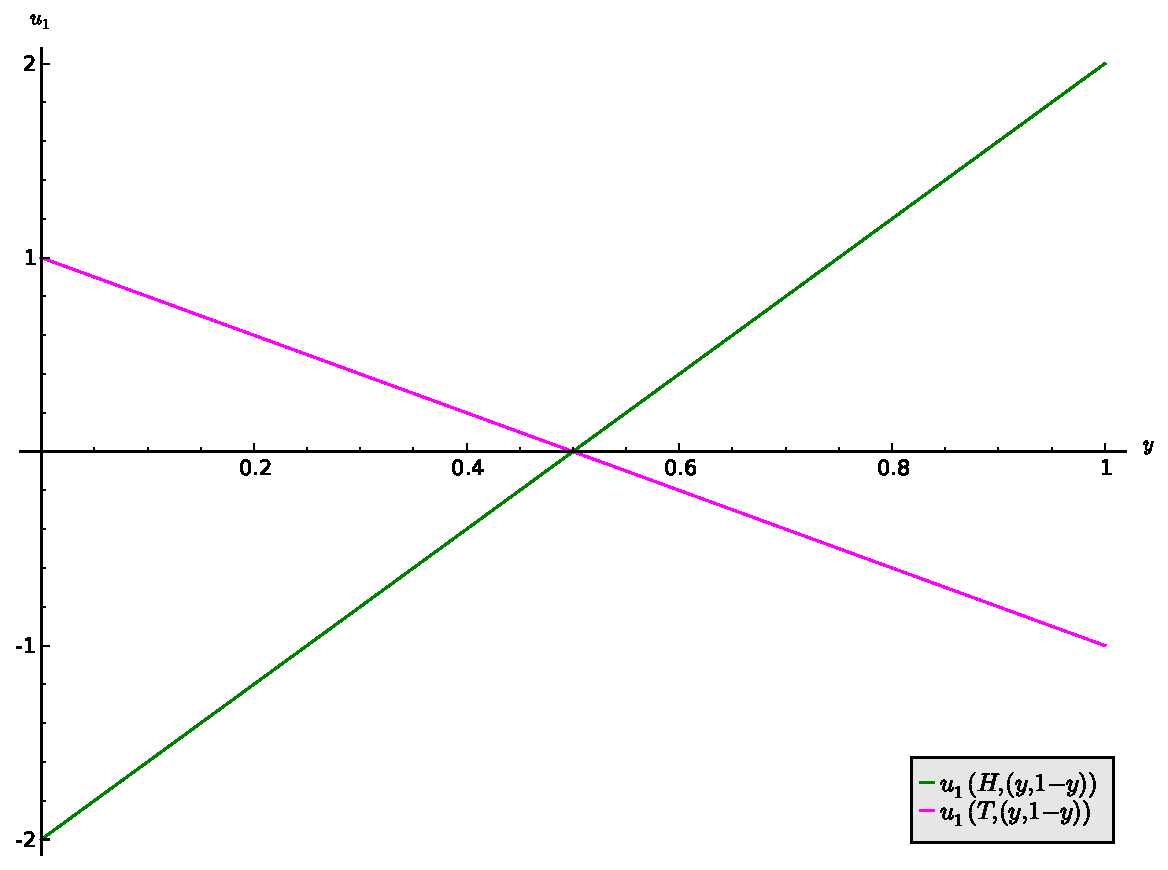
\includegraphics[width=.6\textwidth]{Images/mixedequilibria.pdf}
\end{center}
}

\frame{
\begin{columns}
\column{.5\textwidth}
Row player:
$$s^*_1=\begin{cases}
T\only<2->{\Leftrightarrow x=0},&\text{ if }y<1/2\\
H\only<2->{\Leftrightarrow x=1},&\text{ if }y>1/2\\
\text{Indifferent},&\text{ if }y=1/2\\
\end{cases}$$
\only<3->{
\column{.5\textwidth}
Column player:
$$s^*_2=\begin{cases}
H\only<4>{\Leftrightarrow y=1},&\text{ if }x<1/3\\
T\only<4>{\Leftrightarrow y=0},&\text{ if }x>1/3\\
\text{Indifferent},&\text{ if }x=1/3\\
\end{cases}$$}
\only<1-2>{
\begin{center}
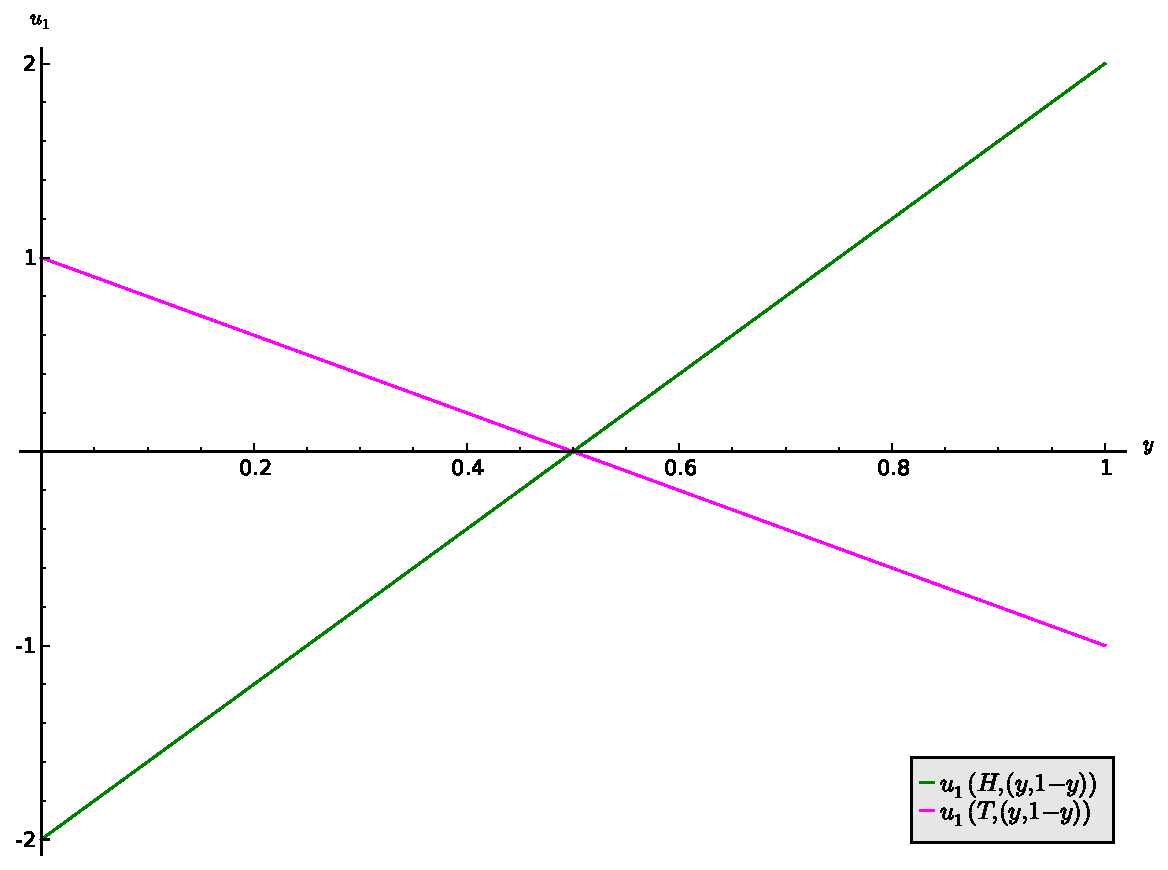
\includegraphics[width=\textwidth]{Images/mixedequilibria.pdf}
\end{center}
}
\end{columns}
}

\end{document}
